
\section{\label{sec:RootsBracketing}Pengurungan\index{pengurungan}}

Metode bagi dua disebut metode pencarian akar dengan pengurungan.
Sebuah akar diketahui berada di dalam suatu selang tertentu. Setiap
iterasi memperkecil lebar selang sambil mempertahankan jaminan bahwa
akar tetap berada di dalamnya. Pada setiap langkah algoritme, akar
diketahui berada di antara hampiran terbaru dan salah satu hampiran
sebelumnya. Kedua batas ini membentuk selang pengurung bagi akar.
Seiring berjalannya algoritme, lebar selang pengurung menyusut hingga
lebih kecil daripada toleransi tertentu; pada saat itu akar diketahui
sudah dekat dan algoritme berhenti.

Kelemahan metode bagi dua adalah orde kekonvergenannya yang linear.
Dibandingkan dengan metode superlinear seperti metode sekan dan metode
Newton, metode bagi dua bergerak sangat lambat. Namun, metode bagi
dua memiliki sesuatu yang tidak dimiliki metode sekan dan metode Newton---kepastian
kekonvergenan. Memang, metode sekan dan metode Newton cepat ketika
konvergen, tetapi tidak ada jaminan bahwa keduanya akan konvergen.

Metode yang menggabungkan keunggulan metode bagi dua (kekonvergenan
terjamin) dengan metode berorde lebih tinggi (kecepatan) disebut metode
berpengaman. Metode tersebut dijamin konvergen dan dapat melakukannya
dengan cepat ketika hampiran sudah dekat dengan akar. Setiap metode
superlinear dapat dilengkapi dengan pengurungan sehingga menghasilkan
metode berpengaman.

\subsection{Pengurungan}

Pengurungan berarti mempertahankan suatu selang yang diketahui memuat
akar. Pengurungan digunakan dalam metode bagi dua. Pada setiap iterasi,
akar diketahui berada di antara dua hampiran terbaru. Pengurungan
tidak digunakan dalam metode sekan maupun metode Newton. Tidak ada
jaminan bahwa akar tetap dekat dengan hampiran-hampiran terbaru. 

Meskipun demikian, tidaklah sulit untuk menggabungkan metode bagi
dua dengan metode sekan, metode Newton, atau metode berorde tinggi
lainnya, guna membentuk metode hibrida yang menjaga akar tetap terkurung
sekaligus membuka peluang bagi kekonvergenan cepat. Dalam metode seperti
ini, kandidat hampiran berikutnya dihitung menurut metode berorde
tinggi. Jika kandidat berada di dalam selang pengurung, kandidat itu
menjadi hampiran berikutnya. Jika kandidat berada di luar selang pengurung,
metode bagi dua digunakan untuk menghitung hampiran berikutnya sebagai
gantinya.

Metode sekan terkurung\index{metode sekan terkurung}, yang lebih
dikenal sebagai metode posisi palsu atau regula falsi, memberikan
contoh sederhana. Bahkan, metode berorde tinggi (metode sekan) selalu
menghasilkan nilai di dalam selang pengurung, sehingga titik tersebut
tidak perlu diperiksa. Perbedaan antara posisi palsu dan metode sekan
terletak pada pemilihan salah satu dari dua hampiran sebelumnya yang
akan dipertahankan. Dalam metode sekan, hampiran terbarulah yang selalu
dipertahankan untuk langkah berikutnya. Dalam posisi palsu, hampiran
yang mempertahankan selang pengurung bagi akar dipertahankan untuk
langkah berikutnya, baik hampiran itu yang paling baru maupun bukan.
Metode Newton terkurung\index{metode Newton terkurung} memberikan
contoh yang sedikit lebih lanjut karena sangat mungkin hampiran yang
dihasilkan metode Newton jatuh di luar selang pengurung.

Ambil fungsi $g(x)=3-x-\sin(x)$ pada selang $[2,3]$. $f$ kontinu
pada $[2,3]$, dan $g(2)\approx0.09$ serta $g(3)\approx-0.14$ berlainan
tanda. Jadi, $[2,3]$ mengurung sebuah akar $g$; karena itu, tetapkan
$x_{0}=2$ dan $x_{1}=3$. Tabel berikut menunjukkan perhitungan hampiran
berikutnya untuk metode sekan terkurung dan metode Newton terkurung.

\begin{center}
\begin{tabular}{c|cccc}
 & $x_{0}$ & $x_{1}$ & kandidat $x_{2}$ & $x_{2}$\tabularnewline
\hline 
sekan terkurung & $2$ & $3$ & $x_{1}-g(x_{1})\frac{x_{1}-x_{0}}{g(x_{1})-g(x_{0})}\approx2.3912$ & $2.3912$\tabularnewline
Newton terkurung & $2$ & $3$ & $x_{1}-\frac{g(x_{1})}{g'(x_{1})}\approx-11.101$ & $2.5$\tabularnewline
\end{tabular}
\par\end{center}

\noindent Dalam metode sekan terkurung, kandidat $x_{2}$ diterima,
tetapi dalam metode Newton terkurung, kandidat $x_{2}$ berada di
luar selang pengurung sehingga dibuang, dan $x_{2}$ menurut metode
bagi dua ($2.5$) digunakan sebagai gantinya.

Untuk menyiapkan hampiran berikutnya, $g(x_{2})$ dihitung. Karena
$g(x_{2})$ bernilai negatif pada kedua metode, $x_{1}$ lama, yaitu
$3$, dibuang dan $x_{0}=2$ ``dipromosikan'' menjadi $x_{1}$ untuk
mempertahankan selang pengurung. Dengan cara ini, $g$ berlainan tanda
di $x_{1}$ dan $x_{2}$. Tabel berikut memperlihatkan proses pengambilan
keputusan ini sekaligus perhitungan hampiran berikutnya.

\begin{center}
\begin{tabular}{c|ccccc}
 & $g(x_{2})$ & $x_{1}$ & $x_{2}$ & kandidat $x_{3}$ & $x_{3}$\tabularnewline
\hline 
sekan terkurung & $-0.073141$ & $2$ & $2.3912$ & $x_{2}-g(x_{2})\frac{x_{2}-x_{1}}{g(x_{2})-g(x_{1})}\approx2.2165$ & $2.2165$\tabularnewline
Newton terkurung & $-0.098472$ & $2$ & $2.5$ & $x_{2}-\frac{g(x_{2})}{g'(x_{2})}\approx2.0048$ & $2.0048$\tabularnewline
\end{tabular}
\par\end{center}

\noindent Dapatkah Anda melengkapi nilai $x_{4}$ berdasarkan nilai-nilai
dalam tabel berikut? Perhatikan bahwa $x_{1}$ lama harus ``dipromosikan''
pada metode sekan terkurung, tetapi tidak pada metode Newton terkurung.
Mengapa? Jawaban \vpageref{ans:bracketedx4}.

\begin{center}
\begin{tabular}{c|ccccc}
 & $g(x_{3})$ & $x_{2}$ & $x_{3}$ & kandidat $x_{4}$ & $x_{4}$\tabularnewline
\hline 
sekan terkurung & $-0.015215$ & $2$ & $2.2165$ & $x_{3}-g(x_{3})\frac{x_{3}-x_{2}}{g(x_{3})-g(x_{2})}\approx2.1854$ & ?\tabularnewline
Newton terkurung & $0.087906$ & $2.5$ & $2.0048$ & $x_{3}-\frac{g(x_{3})}{g'(x_{3})}\approx2.1565$ & ?\tabularnewline
\end{tabular}
\par\end{center}

\noindent 5 hampiran berikutnya dari setiap metode diberikan di sini
jika Anda ingin mencoba menghitung beberapa di antaranya sendiri.
Sekarang adalah saat yang tepat untuk melakukannya. Nilai-nilai ini
dihitung menggunakan kode Octave berikut.

\begin{center}
\begin{tabular}{c|cc}
 & \multicolumn{2}{c}{terkurung}\tabularnewline
 & sekan & Newton\tabularnewline
\hline 
$x_{5}$ & $2.18062942638407$ & $2.17925592233708$\tabularnewline
$x_{6}$ & $2.17988957044102$ & $2.17975682599184$\tabularnewline
$x_{7}$ & $2.17977718322867$ & $2.17975706647997$\tabularnewline
$x_{8}$ & $2.17976012038625$ & $2.17975706648003$\tabularnewline
$x_{9}$ & $2.17975753008587$ & $2.17975706648003$\tabularnewline
\end{tabular}
\par\end{center}

\subsubsection{Kode Octave untuk Posisi Palsu (Metode Sekan Terkurung)\index{metode sekan terkurung!kode Octave}}

\noindent\begin{verbatim}
%%%%%%%%%%%%%%%%%%%%%%%%%%%%%%%%%%%%%%%%%%%%%%%%%
% Written by Dr. Len Brin           20 May 2014 %
% Purpose: Implementation of the Method of      %
%        False Position.                        %
% INPUT: function g; initial values a and b;    %
%        tolerance TOL; maximum iterations N    %
% OUTPUT: approximation x and number of         %
%        iterations i; or message of failure    %
%%%%%%%%%%%%%%%%%%%%%%%%%%%%%%%%%%%%%%%%%%%%%%%%%
function [x,i] = falsePosition(g,a,b,TOL,N)
  i=1;
  A=g(a);
  B=g(b);
  while (i<N)
    b
    x=b-B*(b-a)/(B-A);
    if (abs(x-b)<TOL)
      return
    end%if
    X=g(x);
    if ((B<0 && X>0) || (B>0 && X<0))
      a=b; A=B;
    end%if
    b=x; B=X;
    i=i+1;
  end%while
  x="Method failed---maximum number of iterations reached";
end%function
\end{verbatim}

\subsubsection{Kode Octave untuk Metode Newton Terkurung\index{metode Newton terkurung!kode Octave}}

\noindent\begin{verbatim}
%%%%%%%%%%%%%%%%%%%%%%%%%%%%%%%%%%%%%%%%%%%%%%%%%
% Written by Dr. Len Brin           20 May 2014 %
% Purpose: Implementation of bracketed Newton's %
%        method.                                %
% INPUT: function g; its derivative gp; initial %
%        values a and b; tolerance TOL; maximum %
%        iterations N                           %
% OUTPUT: approximation x and number of         %
%        iterations i; or message of failure    %
%%%%%%%%%%%%%%%%%%%%%%%%%%%%%%%%%%%%%%%%%%%%%%%%%
function [x,i] = bracketedNewton(g,gp,a,b,TOL,N)
  i=1;
  A=g(a);
  B=g(b);
  while (i<N)
    b
    x=b-B/gp(b);
    if (x<min([a,b]) || x>max([a,b]))
      x=b+(a-b)/2;
    end%if
    if (abs(x-b)<TOL)
      return
    end%if
    X=g(x);
    if ((B<0 && X>0) || (B>0 && X<0))
      a=b; A=B;
    end%if
    b=x; B=X;
    i=i+1;
  end%while
  x="Method failed---maximum number of iterations reached";
end%function
\end{verbatim}\texttt{falsePosition.m} dan \texttt{bracketedNewton.m} dapat diunduh
dari \href{http://lqbrin.github.io/tea-time-numerical/ancillaries.html}{situs pendamping}.

Kode untuk metode sekan terkurung dan metode Newton terkurung sangat
mirip. Bahkan, keduanya hampir identik. Hanya ada dua perbedaan selain
komentar pada bagian awal. Metode sekan terkurung menggunakan baris
\texttt{x=b-B{*}(b-a)/(B-A);}, sedangkan metode Newton terkurung menggunakan
baris \texttt{x=b-B/gp(b);}. Inilah perbedaan mendasar antara keduanya
karena pada bagian inilah metode berorde tinggi dijalankan. Satu-satunya
perbedaan lain adalah metode Newton terkurung menyertakan tiga baris
yang memeriksa apakah \texttt{x} berada di dalam selang pengurung
dan menjalankan satu langkah metode bagi dua jika tidak:

\noindent\begin{verbatim}
    if (x<min([a,b]) || x>max([a,b]))
      x=b+(a-b)/2;
    end%if
\end{verbatim}

\noindent Sebenarnya, kita dapat menambahkan ketiga baris ini ke metode
sekan terkurung dan program akan berjalan sama saja. Metode sekan
tidak mungkin menghasilkan nilai \texttt{x} di luar selang pengurung,
sehingga langkah bagi dua tidak akan pernah dijalankan. Satu-satunya
perbedaan mendasar antara kedua fungsi adalah pelaksanaan metode berorde
tinggi.

Kita dapat menggunakan pengamatan ini untuk membuat semacam cetak
biru bagi pengurungan metode berorde tinggi apa pun. Metode Steffensen,
metode M�ller (selama hampiran tetap riil), atau metode Sidi (Bagian
\ref{sec:polynomialLagrange}), misalnya, dapat diberi pengurungan
dengan cara ini. Kode semu-semu berikut menyajikan cetak biru tersebut
dan memberi panduan untuk mengamankan metode berorde tinggi dengan
menggabungkannya dengan metode bagi dua.

\noindent\begin{pseudocode}\label{pseudo:safeguarded}\index{pengurungan!kode semu}
\begin{description}
\item [{Asumsi:}] $g$ kontinu pada $[a,b]$. $g(a)$ dan $g(b)$ berlainan
tanda.
\item [{Masukan:}] Selang $[a,b]$; fungsi $g$; akurasi yang diinginkan
$tol$; jumlah maksimum iterasi $N$; variabel lain yang diperlukan
untuk menjalankan iterasi metode superlinear, seperti $g'$ dalam
metode Newton.
\item [{Langkah~1:}] Tetapkan $A=g(a)$; $B=g(b)$; $i=2$;
\item [{Langkah~2:}] Inisialisasikan variabel lain yang diperlukan untuk
superlinear();
\item [{Langkah~3:}] Selama $i<N$, lakukan Langkah 4--10:

\begin{description}
\item [{Langkah~4:}] Tetapkan $x=\mbox{superlinear}(a,b,g,\ldots)$;
\item [{Langkah~5:}] Jika $(x-a)(x-b)>0$, maka $x=b+\frac{a-b}{2}$;
\item [{Langkah~6:}] Jika $|x-b|<tol$, kembalikan $x$
\item [{Langkah~7:}] Tetapkan $X=g(x)$;
\item [{Langkah~8:}] Jika $BX<0$, tetapkan $a=b$; $A=B$;
\item [{Langkah~9:}] Tetapkan $b=x$; $B=X$; $i=i+1$;
\item [{Langkah~10:}] Perbarui variabel lain yang diperlukan untuk superlinear();
\end{description}
\item [{Langkah~11:}] Cetak ``Metode gagal. Jumlah maksimum iterasi terlampaui.''
\item [{Keluaran:}] Hampiran $m$ yang berjarak kurang dari $tol$ dari
akar eksak, atau pesan kegagalan.
\end{description}
\end{pseudocode}

Sebagai alasan perlunya mengembangkan versi metode orde tinggi lain
yang memakai selang pengurung, perhatikan fungsi yang sangat bermasalah
$g(x)=\frac{1+10x}{1-10x}$. Fungsi ini berakar di $-\frac{1}{10}$,
tetapi metode sekan dengan selang pengurung dapat sangat lambat konvergen
menuju akar ini. Gambar \ref{fig:troubleForSecant} 
\begin{figure}
\caption{\label{fig:troubleForSecant}Fungsi yang menyulitkan metode sekan
dengan selang pengurung.}

\centering{}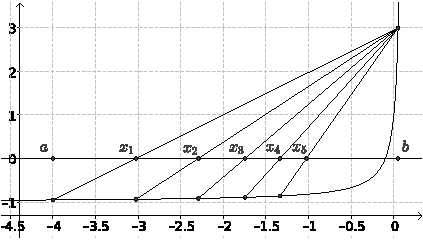
\includegraphics{figures/rootBracketing01}
\end{figure}
 memperlihatkan kekonvergenan lambat ini jika dimulai dengan selang
pengurung $[a,b]=[-4,.05]$. Dengan pilihan selang pengurung yang
kurang tepat ini, metode membutuhkan 45 iterasi untuk mencapai akurasi
$10^{-5}$. Algoritma yang lebih cerdas tidak hanya memeriksa bahwa
setiap hampiran berada di dalam selang pengurung, tetapi juga memastikan
bahwa metode orde tinggi bergerak cukup cepat menuju akar. Jika algoritma
mendeteksi kekonvergenan yang lambat, misalnya lebih lambat daripada
metode bagi dua, algoritma akan menggunakan langkah bagi dua sebagai
gantinya. Perhatikan bahwa metode Newton dengan selang pengurung tidak
mengalami masalah berarti pada fungsi ini. Dengan selang pengurung
awal yang sama, metode tersebut mencapai jarak $10^{-5}$ dari akar
hanya dalam 10 iterasi (empat iterasi pertamanya merupakan langkah
bagi dua). Sayangnya, metode Newton memerlukan turunan. Metode cepat
untuk mencari akar dalam selang pengurung tanpa memerlukan turunan
akan sangat berguna.

Pada awal 1970-an, Richard Brent\index{metode Brent}\index{metode!Brent|see{metode Brent}}
mengembangkan karya van Wijngaarden dan Dekker menjadi metode dengan
selang pengurung yang memadukan metode bagi dua, metode sekan, dan
interpolasi kuadratik invers, sambil terus memeriksa bahwa metode
orde tinggi bergerak cukup cepat menuju akar. Hasilnya kini dikenal
sebagai metode Brent \cite{brent}. Metode ini tidak memerlukan turunan.
Metode ini cepat. Kekonvergenannya dijamin. Karena itu, metode ini
populer sebagai metode serbaguna untuk mencari akar dalam selang pengurung
ketika turunan tidak tersedia. Rincian lengkap metode Brent tidak
akan disajikan di sini, tetapi satu langkah penting menuju metode
tersebut akan disajikan. Metode yang disajikan di sini mirip dengan
fungsi MATLAB \texttt{fzero} \cite{moler}.

\subsection{Interpolasi Kuadratik Invers\index{metode interpolasi kuadratik invers}}

Seperti yang mungkin Anda ingat, metode M�ller memerlukan tiga hampiran
awal, misalnya $a$, $b$, dan $c$. Parabola yang melalui titik $(a,g(a))$,
$(b,g(b))$, dan $(c,g(c))$ digambar, dan titik potongnya dengan
sumbu $x$ menghasilkan hampiran berikutnya. Unsur kunci metode ini---proses
mencocokkan fungsi kuadrat dengan ketiga titik---disebut interpolasi.
Dengan demikian, metode M�ller juga dapat disebut ``metode interpolasi
kuadratik''.

Seperti dapat diduga, metode interpolasi kuadratik invers serupa.
Alih-alih mencocokkan fungsi kuadrat dengan titik $(a,g(a))$, $(b,g(b))$,
dan $(c,g(c))$, peran $x$ dan $y$ dipertukarkan. Sebagai gantinya,
fungsi kuadrat dicocokkan dengan titik $(g(a),a)$, $(g(b),b)$, dan
$(g(c),c)$. Karena dalam kasus ini $x$ merupakan fungsi dari $y$,
grafik fungsi kuadrat itu akan memotong sumbu $x$ tepat sekali, yakni
saat $y=0$. Mengevaluasi fungsi kuadrat di $0$ menghasilkan hampiran
berikutnya. Gambar \ref{fig:quadraticVSinverseQuadratic} memperlihatkan
interpolasi kuadratik dan interpolasi kuadratik invers pada himpunan
tiga titik yang sama. Dalam interpolasi kuadratik, $y$ diperlakukan
sebagai fungsi dari $x$. Dalam interpolasi kuadratik invers, $x$
diperlakukan sebagai fungsi dari $y$. Interpolasi kuadratik invers
menghindari komplikasi utama interpolasi kuadratik---menghitung titik
potongnya dengan sumbu $x$. Dalam interpolasi kuadratik, fungsi kuadrat
mungkin memotong sumbu $x$ dua kali atau sama sekali tidak memotongnya!
Dalam kedua kasus, suatu pilihan harus dibuat pada setiap langkah,
dan akar-akar fungsi kuadrat melibatkan rumus kuadrat. Dalam interpolasi
kuadratik invers, fungsi kuadrat dijamin memotong sumbu $x$ tepat
sekali, dan titik potong itu cukup dicari dengan mengevaluasi fungsi
kuadrat di $0$. Artinya, $y=0$. Ingat, fungsi kuadrat memberikan
$x$ sebagai fungsi dari $y$.

Dengan merujuk kembali pada penurunan metode M�ller \vpageref{subsec:mullers},
jika parabola dipaksa melalui titik $(a,A)$, $(b,B)$, dan $(c,C)$,
lalu peran $x$ dan $y$ dipertukarkan, rumus untuk parabola invers
$q$ langsung diperoleh:

\[
q(y)=q_{0}(y-B)^{2}+q_{1}(y-B)+q_{2}
\]
dengan
\begin{eqnarray*}
q_{2} & = & b\\
q_{1} & = & \frac{(A-B)^{2}(c-b)-(C-B)^{2}(a-b)}{(A-B)(C-B)(A-C)}\\
q_{0} & = & \frac{(C-B)(a-b)-(A-B)(c-b)}{(A-B)(C-B)(A-C)}.
\end{eqnarray*}
\begin{digression}{Orde kekonvergenan interpolasi kuadratik} 

\noindent Metode interpolasi kuadratik invers\index{metode interpolasi kuadratik invers!orde kekonvergenan}
memiliki orde kekonvergenan sekitar $1.84$ dengan asumsi yang wajar.
Jika fungsi yang akarnya dicari memiliki tiga turunan kontinu di suatu
lingkungan akar, tiga hampiran terbaru cukup dekat, dan akarnya sederhana,
orde kekonvergenannya adalah solusi riil dari 
\[
\alpha^{3}-\alpha^{2}-\alpha-1=0.
\]
Kita dapat menggunakan interpolasi kuadratik invers untuk menghampirinya!
\begin{verbatim}
>> format('long')
>> f=@(x) x^3-x^2-x-1
f =
@(x) x ^ 3 - x ^ 2 - x - 1
>> [res,i]=inverseQuadratic(f,1,2,10^-12,100)
res =  1.83928675521416
i =  8
\end{verbatim} Solusi eksaknya adalah
\[
\alpha=\left(\frac{\sqrt{11}}{3\sqrt{3}}+\frac{19}{27}\right)^{\frac{1}{3}}+\frac{4}{9\left(\frac{\sqrt{11}}{3\sqrt{3}}+\frac{19}{27}\right)^{\frac{1}{3}}}+\frac{1}{3}.
\]
Anda mungkin mengenali nilai ini sebagai orde kekonvergenan metode
M�ller. Memang, setiap metode interpolasi kuadratik konvergen menuju
akar sederhana dengan orde ini.
\begin{description}
\item [{Referensi}] \cite{sharma}
\end{description}
\noindent\end{digression} 

Dengan demikian, titik potong dengan sumbu $x$ adalah 
\begin{eqnarray*}
x & = & q(0)\\
 & = & B^{2}q_{0}-Bq_{1}+q_{2}\\
 & = & B^{2}\frac{(C-B)(a-b)-(A-B)(c-b)}{(A-B)(C-B)(A-C)}-B\frac{(A-B)^{2}(c-b)-(C-B)^{2}(a-b)}{(A-B)(C-B)(A-C)}+b\\
 & = & \frac{\left[B^{2}(C-B)+B(C-B)^{2}\right](a-b)-\left[B^{2}(A-B)+B(A-B)^{2}\right](c-b)}{(A-B)(C-B)(A-C)}+b\\
 & = & \frac{\left[-B^{2}C+BC^{2}\right](a-b)-\left[-B^{2}A+BA^{2}\right](c-b)}{(A-B)(C-B)(A-C)}+b\\
 & = & \frac{BC(C-B)(a-b)-BA(A-B)(c-b)}{(A-B)(C-B)(A-C)}+b\\
 & = & b+\frac{\frac{B}{A}(\frac{C}{B}-1)(a-b)-\frac{A}{C}(1-\frac{B}{A})(c-b)}{(1-\frac{B}{A})(\frac{C}{B}-1)(\frac{A}{C}-1)}\\
 & = & b+\frac{\frac{A}{C}(1-\frac{B}{A})(c-b)-\frac{B}{A}(\frac{C}{B}-1)(a-b)}{(\frac{B}{A}-1)(\frac{B}{C}-1)(\frac{A}{C}-1)}.
\end{eqnarray*}
Agar perhitungan $x$ sedikit lebih mudah diprogram, diperkenalkan
beberapa variabel baru. Misalkan
\[
r=\frac{B}{A}-1,\quad s=\frac{C}{B}-1,\quad t=\frac{A}{C}-1
\]
sehingga
\begin{equation}
x=b-\frac{r(t+1)(c-b)+s(r+1)(a-b)}{rst}.\label{eq:inverseQuadratic}
\end{equation}

\begin{figure}
\caption{\label{fig:quadraticVSinverseQuadratic}Interpolasi kuadratik dan
interpolasi kuadratik invers.}

\centering{}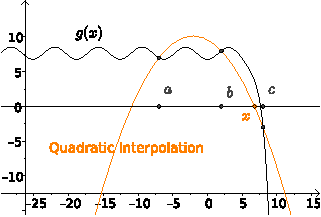
\includegraphics{figures/rootBracketing02}\qquad{}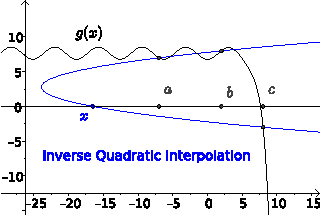
\includegraphics{figures/rootBracketing03}
\end{figure}

Interpolasi kuadratik invers dapat dilengkapi selang pengurung seperti
metode orde tinggi lainnya. Namun, metode ini menimbulkan pertanyaan
menarik yang tidak muncul pada semua metode orde tinggi. Interpolasi
kuadratik memerlukan tiga titik; ketika ketiganya digunakan untuk
menghasilkan hampiran berikutnya, terbentuk titik keempat. Dari keempat
titik itu, komputer harus menentukan dua titik yang akan menjadi selang
pengurung berikutnya dan satu titik yang akan menjadi titik ketiga
untuk interpolasi berikutnya. Namun, kita sudah melangkah terlalu
jauh.

Setiap iterasi dimulai dengan tiga titik, $(a,g(a))$, $(b,g(b))$,
dan $(c,g(c))$, dengan $a$ dan $b$ mengurung sebuah akar, sedangkan
$c$ merupakan titik ketiga. Pada iterasi pertama, hanya selang pengurung
yang diberikan. $c$ disamakan dengan $a$. Pada setiap iterasi, tanda
$g(a)$ dan $g(b)$ diperiksa untuk memastikan bahwa $a$ dan $b$
mengurung sebuah akar. Jika tandanya berlainan, metode dilanjutkan.
Jika tandanya sama, berarti $g(b)$ dan $g(c)$ pasti berlainan tanda,
sehingga $a$ disamakan dengan $c$. Selanjutnya, nilai mutlak $g(a)$
dan $g(b)$ diperiksa. Jika $|g(a)|<|g(b)|$, label $a$ dan $b$
dipertukarkan dan $c$ disamakan dengan nilai baru $a$. Setelah pemeriksaan
awal ini, perhitungan hampiran berikutnya dimulai dengan jaminan bahwa
sebuah akar terletak di antara $a$ dan $b$; $b$ kemungkinan merupakan
taksiran akar terbaik sejauh ini; dan $c$ kemungkinan merupakan taksiran
akar terburuk sejauh ini.

Jika $c=a$ setelah pemeriksaan awal dan kemungkinan pelabelan ulang,
interpolasi kuadratik tidak dapat dilakukan. Hampiran berikutnya dihasilkan
dengan metode sekan (interpolasi linear). Jika $c\neq a$ setelah
pemeriksaan awal dan kemungkinan pelabelan ulang, calon hampiran berikutnya,
$x$, dihitung menggunakan interpolasi kuadratik invers. Jika calon
tersebut berada di dalam selang pengurung, calon itu diterima sebagai
hampiran berikutnya. Jika berada di luar selang pengurung, langkah
metode bagi dua digunakan sebagai gantinya. Dalam kedua kasus, $c$
disamakan dengan $b$ dan $b$ disamakan dengan $x$. Untuk interpolasi
kuadratik invers dengan selang pengurung, hal ini menuntaskan satu
iterasi. Metode kemudian diulang sampai ditemukan hampiran yang cukup
baik.

Dalam skenario terbaik, interpolasi kuadratik invers digunakan pada
setiap langkah dan kekonvergenannya superlinear dengan orde sekitar
$1.84$. Dalam skenario terburuk, salah satu metode orde tinggi digunakan
pada setiap langkah, tetapi fungsinya patologis dan kekonvergenannya
lambat, bahkan mungkin lebih lambat daripada metode bagi dua. Meskipun
demikian, kekonvergenan lambat jarang terjadi, dan orde kekonvergenan
aktual secara umum tidak dapat ditentukan secara pasti. Metode ini
berganti-ganti antara metode yang berbeda orde. Yang dapat kita katakan
hanyalah bahwa biasanya metode ini cepat.

\subsubsection{Kode Octave untuk Interpolasi Kuadratik Invers dengan Selang Pengurung\index{interpolasi kuadratik invers dengan selang pengurung!kode Octave}}

\begin{verbatim}
%%%%%%%%%%%%%%%%%%%%%%%%%%%%%%%%%%%%%%%%%%%%%%%%%
% Written by Dr. Len Brin           21 May 2014 %
% Purpose: Implementation of bracketed inverse  %
%        quadratic interpolation method.        %
% INPUT: function g; initial values a and b;    %
%        tolerance TOL; maximum iterations N0   %
% OUTPUT: approximation x and number of         %
%        iterations i; or message of failure    %
%%%%%%%%%%%%%%%%%%%%%%%%%%%%%%%%%%%%%%%%%%%%%%%%%
function [x,i] = bracketedInverseQuadratic(g,a,b,TOL,N0)
  i=1;
  A=g(a);
  B=g(b);
  c=a; C=A;
  while (i<N0)
    b
    if (B*A>0)
      a=c; A=C;
    end%if
    if (abs(A) < abs(B))
      c=b; C=B;
      b=a; B=A;
      a=c; A=C;
    end%if
    if (a==c)
      x=(b*A-a*B)/(A-B);
    else
      r=B/A-1; s=C/B-1; t=A/C-1;
      p=(t+1)*r*(c-b)+(r+1)*s*(a-b);
      q=t*s*r;
      x=b-p/q;
    end%if
    if (x<min([a,b]) || x>max([a,b]))
      x=b+(a-b)/2;
    end%if
    if (abs(x-b)<TOL)
      disp(" ");
      return
    end%if
    c=b; C=B;
    b=x; B=g(b);
    i=i+1;
  end%while
  x="Method failed---maximum number of iterations reached";
end%function
\end{verbatim} Penerapan metode interpolasi kuadratik invers dengan selang pengurung
pada fungsi bermasalah $g(x)=\frac{1+10x}{1-10x}$ di selang $[-4,.05]$
menghasilkan akurasi $10^{-5}$ hanya dalam 11 iterasi. Metode ini
hanya membutuhkan satu iterasi lebih banyak daripada metode Newton
dengan selang pengurung, tanpa memerlukan turunan $g$! \texttt{bracketedInverseQuadratic.m}
dapat diunduh dari \href{http://lqbrin.github.io/tea-time-numerical/ancillaries.html}{situs pendamping}.

\subsection{Penghentian\index{kriteria penghentian!untuk pencarian akar}}

Dalam semua metode pencarian akar kita, algoritme berhenti ketika
selisih antara dua hampiran berturut-turut lebih kecil daripada toleransi
tertentu. Kriteria ini didasarkan pada asumsi bahwa galat tidak akan
melebihi selisih tersebut. Asumsi itu aman bagi setiap metode yang
sedang konvergen secara superlinear ketika berhenti. Bahkan, asumsi
itu juga aman bagi metode bagi dua yang konvergen secara linear, karena
selisih antara dua hampiran berturut-turut tepat sama dengan batas
teoretis galat. 

Kriteria ini tidak aman ketika metode superlinear digunakan begitu
jauh dari akar sehingga kekonvergenan superlinear tidak tampak. Inilah
tepatnya yang terjadi pada Gambar \vpageref{fig:troubleForSecant}.
Selisih antara hampiran-hampiran berturut-turut sebenarnya lebih besar
daripada galat absolut pada setiap langkah. Situasi ini tidak lazim,
tetapi dapat terjadi. 

Kriteria ini juga tidak aman ketika suatu metode konvergen secara
linear dengan konstanta kekonvergenan asimtotik $\lambda>\frac{1}{2}$.
Namun, metode yang konvergen secara linear sebaiknya tidak pernah
digunakan sendiri karena selalu ada alternatif yang lebih cepat.

Ada satu pertimbangan penting lagi mengenai penghentian. Berhenti
ketika selisih antara dua hampiran berturut-turut lebih kecil daripada
toleransi tertentu bergantung pada galat absolut. Ketika akar mungkin
sangat kecil atau sangat besar, barangkali lebih baik menggunakan
kriteria berdasarkan galat relatif. Sebagai contoh, alih-alih berhenti
ketika $|x_{n+1}-x_{n}|<tol$, kita berhenti ketika $|x_{n+1}-x_{n}|<tol\cdot|x_{n+1}|$.

\subsection{Konsep Kunci}
\begin{description}
\item [{Pengurungan:}] \index{pengurungan}Memperhalus secara iteratif
suatu selang---yang juga disebut selang pengurung---yang diketahui
memuat akar, hingga lebarnya lebih kecil daripada toleransi tertentu.
\item [{Interpolasi~kuadratik~invers:}] \index{metode interpolasi kuadratik invers}\index{metode!interpolasi kuadratik invers|see{metode interpolasi kuadratik invers}}Sebuah
polinom kuadrat dalam $y$ dicocokkan dengan tiga hampiran akar berturut-turut.
Titik potong kurva kuadratik dengan sumbu $x$ menjadi hampiran berikutnya.
\item [{Metode~sekan~terkurung:}] \index{metode sekan terkurung}\index{metode!sekan terkurung|see{metode sekan terkurung}}Gabungan
metode sekan dan metode bagi dua yang menggunakan pengurungan. Pada
setiap iterasi, jika metode sekan menghasilkan nilai di dalam selang
pengurung saat ini, nilai itu menjadi hampiran berikutnya. Jika tidak,
metode bagi dua digunakan untuk menghasilkan hampiran berikutnya.
\item [{Posisi~palsu:}] \index{metode!posisi palsu|see{metode sekan terkurung}}\index{posisi palsu|see{metode sekan terkurung}}Nama
lain untuk metode sekan terkurung.
\item [{Regula~falsi:}] \index{metode!regula falsi|see{metode sekan terkurung}}\index{regula falsi|see{metode sekan terkurung}}Nama
lain untuk metode sekan terkurung.
\item [{Metode~Newton~terkurung:}] \index{metode Newton terkurung}\index{metode!Newton terkurung|see{metode Newton terkurung}}Gabungan
metode Newton dan metode bagi dua yang menggunakan pengurungan. Pada
setiap iterasi, jika metode Newton menghasilkan nilai di dalam selang
pengurung saat ini, nilai itu menjadi hampiran berikutnya. Jika tidak,
metode bagi dua digunakan untuk menghasilkan hampiran berikutnya.
\item [{Interpolasi~kuadratik~invers~terkurung:}] \index{interpolasi kuadratik invers terkurung}\index{metode!interpolasi kuadratik invers terkurung|see{interpolasi kuadratik invers terkurung}}Gabungan
interpolasi kuadratik invers, metode sekan, dan metode bagi dua yang
menggunakan pengurungan. Pada setiap iterasi, jika interpolasi kuadratik
invers menghasilkan nilai di dalam selang pengurung saat ini, nilai
itu menjadi hampiran berikutnya. Jika tidak, metode sekan atau metode
bagi dua digunakan untuk menghasilkan hampiran berikutnya.
\end{description}
\noindent\startexercises 

\subsection{Latihan}
\begin{enumerate}
\item \label{exc:bracketing}Gunakan metode sekan terkurung (posisi palsu)
untuk menemukan sebuah akar pada selang yang ditunjukkan, dengan akurasi
hingga $10^{-2}$.

\begin{enumerate}
\item $f(x)=3-x-\sin x$; $[2,3]$ \hasananswer 
\item $g(x)=3x^{4}-2x^{3}-3x+2$; $[0,1]$
\item $g(x)=3x^{4}-2x^{3}-3x+2$; $[0,0.9]$ \hasasolution 
\item $h(x)=10-\cosh(x)$; $[-3,-2]$
\item $f(t)=\sqrt{4+5\sin t}-2.5$; $[-600,-500]$ \hasananswer 
\item $g(t)=\tan\left(\frac{t^{2}}{1-3t}\right)$; $[3486,3487]$
\item $h(t)=\ln(3\sin t)-\frac{3t}{5}$; $[1,2]$
\item $f(r)=e^{\sin r}-r$; $[-20,20]$ \hasasolution 
\item $g(r)=\sin(e^{r})+r$; $[-3,3]$
\item $h(r)=2^{\sin r}-3^{\cos r}$; $[1,3]$ \hasananswer 
\end{enumerate}
\item \label{exc:bracketing-1}Ulangi soal \ref{exc:bracketing} dengan
menggunakan metode Newton terkurung. \haspartwithsolution  \haspartwithanswer 
\item \label{exc:bracketing-2}Ulangi soal \ref{exc:bracketing} dengan
menggunakan metode sekan. Bandingkan jawaban Anda dengan hasil posisi
palsu. \haspartwithsolution  \haspartwithanswer 
\item \label{exc:bracketing-3}Ulangi soal \ref{exc:bracketing} dengan
menggunakan metode Newton. Bandingkan jawaban Anda dengan hasil metode
Newton terkurung. \haspartwithsolution  \haspartwithanswer 
\item \label{exc:bracketing-4}\octave\ Ulangi soal \ref{exc:bracketing}
dengan menggunakan Octave dan toleransi $10^{-6}$. \haspartwithsolution  \haspartwithanswer 
\item \label{exc:bracketing-5}\octave\ Ulangi soal \ref{exc:bracketing-1}
dengan menggunakan Octave dan toleransi $10^{-6}$. \haspartwithsolution  \haspartwithanswer 
\item \label{exc:bracketing-6}\octave\ Ulangi soal \ref{exc:bracketing}
dengan menggunakan Octave, interpolasi kuadratik invers dengan pengurungan,
dan toleransi $10^{-6}$. \haspartwithsolution  \haspartwithanswer 
\item \label{exc:bracketing-7}Bandingkan hasil pada soal \ref{exc:bracketing-4},
\ref{exc:bracketing-5}, dan \ref{exc:bracketing-6}. \haspartwithanswer 
\item \label{exc:bracketing-8}\octave\ Tulislah sebuah fungsi Octave yang
mengimplementasikan metode Steffensen dengan pengurungan. \textbf{CATATAN:}
Metode Steffensen merupakan metode pencarian titik tetap. Metode ini
menyelesaikan persamaan $f(x)=x$, bukan $f(x)=0$. Jadi, selang pengurung
$[a,b]$ yang sah adalah selang yang memenuhi ($f(a)>a$ dan $f(b)<b$)
atau ($f(a)<a$ dan $f(b)>b$). Secara geometris, ini berarti titik-titik
$(a,f(a))$ dan $(b,f(b))$ berada pada sisi berlawanan dari garis
$f(x)=x$, analog dengan selang pengurung pencarian akar yang kedua
titiknya berada pada sisi berlawanan dari garis $f(x)=0$.
\item \label{exc:bracketing-9}\octave\ Gunakan kode Anda dari soal \ref{exc:bracketing-8}
untuk mengulangi soal \ref{exc:bracketing} dengan menggunakan Octave,
metode Steffensen dengan pengurungan, dan toleransi $10^{-6}$. Karena
Anda mencari akar $g(x)$, gunakan $f(x)=g(x)+x$ saat memanggil metode
Steffensen. \haspartwithsolution  \haspartwithanswer 
\item \label{exc:bracketing-13}Bandingkan hasil pada soal \ref{exc:bracketing-6}
dan \ref{exc:bracketing-9}. \haspartwithanswer 
\item \label{exc:bracketing-10}\octave\ Tulislah ulang fungsi Octave \texttt{inverseQuadraticInterpolation}
agar berhenti ketika galat relatif hampiran lebih kecil daripada toleransi.
\item \label{exc:bracketing-11}\octave\ Gunakan kode Anda dari soal \ref{exc:bracketing-10}
untuk mengulangi soal \ref{exc:bracketing} dengan toleransi $10^{-6}$. \haspartwithsolution  \haspartwithanswer 
\item \label{exc:bracketing-14}Bandingkan hasil pada soal \ref{exc:bracketing-6}
dan \ref{exc:bracketing-11}. \haspartwithanswer 
\end{enumerate}
\noindent\finishexercises 

\subsection{Jawaban}
\begin{description}
\item [{$x_{4}$:}] \label{ans:bracketedx4}Pada kedua metode, kandidat
$x_{4}$ diterima karena dalam masing-masing kasus, $x_{4}$ berada
di dalam selang pengurung yang dibentuk oleh $x_{2}$ dan $x_{3}$.
Jadi, untuk metode sekan dengan pengurungan, $x_{4}=2.1854$, sedangkan
untuk metode Newton dengan pengurungan, $x_{4}=2.1565$ Pada metode
sekan dengan pengurungan, . $x_{1}$ diperbarui menjadi $x_{2}$ karena
$g(x_{3})$ bernilai negatif. $g(x_{2})$ dan $g(x_{3})$ harus berlainan
tanda agar selang pengurung tetap terjaga. Pada metode Newton dengan
pengurungan, $x_{1}$ tidak diperbarui karena $g(x_{3})$ bernilai
positif.
\end{description}

